%%%%%%%%%%%%%%%%%%%%%%%%%%%%%%%%%%%%%%%%%
% NIWeek 2014 Poster by T. Reveyrand
% www.microwave.fr
% http://www.microwave.fr/LaTeX.html
% ---------------------------------------
% 
% Original template created by:
% Brian Amberg (baposter@brian-amberg.de)
%
% This template has been downloaded from:
% http://www.LaTeXTemplates.com
%
% License:
% CC BY-NC-SA 3.0 (http://creativecommons.org/licenses/by-nc-sa/3.0/)
%
%%%%%%%%%%%%%%%%%%%%%%%%%%%%%%%%%%%%%%%%%

%----------------------------------------------------------------------------------------
%   PACKAGES AND OTHER DOCUMENT CONFIGURATIONS
%----------------------------------------------------------------------------------------

\documentclass[a0paper,portrait]{baposter}

\usepackage[font=small,labelfont=bf]{caption} % Required for specifying captions to tables and figures
\usepackage{booktabs} % Horizontal rules in tables
\usepackage{relsize} % Used for making text smaller in some places

\usepackage{amsmath,amsfonts,amssymb,amsthm} % Math packages
\usepackage{eqparbox}

\usepackage{textcomp}

\graphicspath{{figures/}} % Directory in which figures are stored

 \definecolor{bordercol}{RGB}{40,40,40} % Border color of content boxes
 \definecolor{headercol1}{RGB}{186,215,230} % Background color for the header in the content boxes (left side)
 \definecolor{headercol2}{RGB}{120,120,120} % Background color for the header in the content boxes (right side)
 \definecolor{headerfontcol}{RGB}{0,0,0} % Text color for the header text in the content boxes
 \definecolor{boxcolor}{RGB}{210,235,250} % Background color for the content in the content boxes


\begin{document}

\background{ % Set the background to an image (background.pdf)
\begin{tikzpicture}[remember picture,overlay]
\draw (current page.north west)+(-2em,2em) node[anchor=north west]
{
\includegraphics[height=1.1\textheight]{background}};
\end{tikzpicture}
}

\begin{poster}{
grid=false,
columns=4,
borderColor=bordercol, % Border color of content boxes
headerColorOne=headercol1, % Background color for the header in the content boxes (left side)
headerColorTwo=headercol2, % Background color for the header in the content boxes (right side)
headerFontColor=headerfontcol, % Text color for the header text in the content boxes
boxColorOne=boxcolor, % Background color for the content in the content boxes
headershape=roundedright, % Specify the rounded corner in the content box headers
headerfont=\Large\sf\bf, % Font modifiers for the text in the content box headers
textborder=rectangle,
background=none,
headerborder=open, % Change to closed for a line under the content box headers
boxshade=plain
}
{
\includegraphics[scale=0.3]{CU.png}}
%
%----------------------------------------------------------------------------------------
%   TITLE AND AUTHOR NAME
%----------------------------------------------------------------------------------------
%
{ \bf  \huge {Generalized LL Parsing Generalization} \\  \Large \it An affordable PXI-based microwave non-linear characterization platform} % Poster title
{\vspace{0.3em} \smaller \textbf{Semyon Grigorev$^1$}, Artem Gorokhov$^1$ \\  % Author names
\smaller \it $^1${Saint Petersburg State University, JetBrains, St. Petersburg, Russia } \\ % Author email addresses
\smaller  {\textbf{E-mail:} semen.grigorev@jetbrains.com}}
{
\includegraphics[scale=0.45]{NI.jpg}} % University/lab logo


%----------------------------------------------------------------------------------------
%   INTRODUCTION
%----------------------------------------------------------------------------------------
\headerbox{Motivation}{name=introduction,column=0,row=0, span=2}{

Nowadays input data for parsing algorithms are not limited to be linear strings, and context-free grammars are used not only for programming languages specification.
One of classical examples is a context-free path querying for graph data bases where input is a graph and path constraints are specified by a grammar.
There are also other generalizations of parsing, such as multiple input GLL parsing presented at Parsing@SLE-2016 by Elizabeth Scott and Adrian Johnstone, 
Abstract LR parsing~\cite{AbstractParsing} and other techniques for parsing of dynamically generated strings.

%
%
%We have some ideas of graph parsing applications.
%For example, context-free pattern search in metagenomical assemblies, which can be applied not only to regular input, but to context-free compressed input which is relevant for metagenomic assembly processing. 
%All existing applications seem to be special cases of the Bar-Hillel~\cite{Bar-Hillel} theorem for context-free and regular language intersection, and can be generalized, but today many of them are developed as stand alone solutions.
Thus, the goal of our work is to create an abstract framework for parsing based on generalization of GLL parsing algorithm~\cite{GLL} proposed by Elizabeth Scott and Adrian Johnstone. 
%We also want to investigate practical areas of application and to create solutions based on our framework to demonstrate its practical value.

}

\headerbox{Results}{name=results,column=2,row=0, span=2}{
\begin{itemize} 
\item GLL-based parsing framework
\vspace{-0.2cm}
\item GLL-based context-free path querying algorithm~\cite{GraphGLL} implemented by the authors is faster than solution which was presented at ISWC-2016~\cite{CFRDFParsing}. 
\vspace{-0.2cm}
\item We have some experience in the areas mentioned above~\cite{GraphGLL, RelaxedRNGLR}.
\end{itemize}
}

\headerbox{Future Research}{name=results,column=2,below=results, span=2}{
\begin{itemize} 
\item Mechanization in Coq
\vspace{-0.2cm}
\item Tool for 
\vspace{-0.2cm}
\item Context-free compressed data processing
\end{itemize}
}

\headerbox{Bar-Hillel Theorem}{name=bh,column=0,below=introduction, span=2}{
All existing applications seem to be special cases of the Bar-Hillel~\cite{Bar-Hillel} theorem for context-free and regular language intersection, and can be generalized, but today many of them are developed as stand alone solutions.
}

\headerbox{Generalized LL}{name=gll,column=2,below=introduction, span=2}{
\begin{itemize} 
\item Arbitrary grammars
\item Cubic time. Linear
\item SPPF as input
\end{itemize}
}

%----------------------------------------------------------------------------------------
%   CALIBRATION
%----------------------------------------------------------------------------------------
\headerbox{Linear input parsing}{name=calibration,column=0,below=gll}{
\begin{itemize}
\item Classical
\item Multilexem
\item Error recovery
\end{itemize}
}

%----------------------------------------------------------------------------------------
%   OTHER INSTRUMENTATION
%----------------------------------------------------------------------------------------
\headerbox{Graph parsing}
{name=grphparsing,column=1,span=1, below=gll}{ % To reduce this block to 1 column width, remove 'span=2'
Graph DB, metagenomic assemblies etc.
}

\headerbox{String-embedded code parsing}
{name=grphparsing,column=2,span=1, below=gll}{ % To reduce this block to 1 column width, remove 'span=2'
Graph DB, metagenomic assemblies etc.
}


\headerbox{CF compression}
{name=cfcompression,column=3,row=1, below=gll}{ % To reduce this block to 1 column width, remove 'span=2'

Compressed data processing
}

%----------------------------------------------------------------------------------------
%   MIXER vs. SAMPLERS
%----------------------------------------------------------------------------------------
\headerbox{Generalized LL generalization}{name=receiver,span=3,column=0,row=1, below=grphparsing}{
All above is graph parsing!
%\begin{center}
%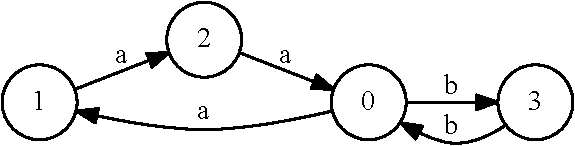
\includegraphics[width=0.5\textwidth]{input.pdf}    \[
%\begin{array}{rl}
%   0:& S \rightarrow a \ S \ b \\
%   1:& S \rightarrow Middle \\
%   2:& Middle \rightarrow a \ b
%\end{array}
%\]

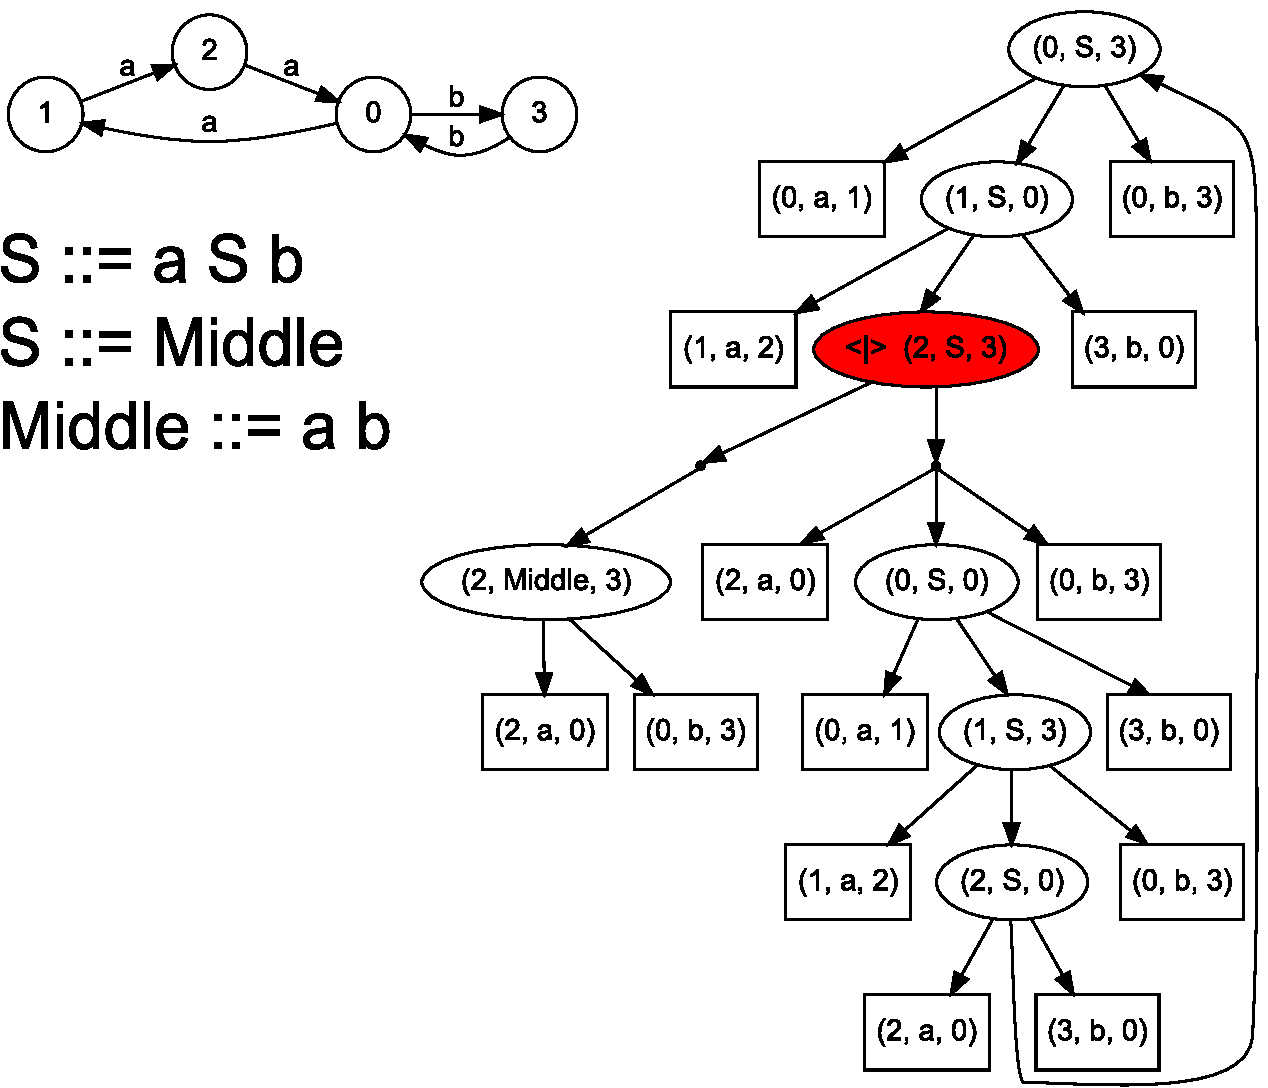
\includegraphics[width=0.9\textwidth]{AnBn_r.pdf}

%\end{center}
}


%----------------------------------------------------------------------------------------
%   REFERENCES
%----------------------------------------------------------------------------------------

\headerbox{References}{name=references,column=2,below=application}{

\smaller % Reduce the font size in this block
\renewcommand{\section}[2]{\vskip 0.05em} % Get rid of the default "References" section title
%\nocite{*} % Insert publications even if they are not cited in the poster

\bibliographystyle{unsrt}
\bibliographystyle{IEEEtran}
\bibliography{biblio} % Use biblio.bib as the bibliography file
}




\end{poster}

\end{document}